\begin{figure}[!ht]
  \begin{subfigure}[t]{0.5\textwidth}
    \centering
    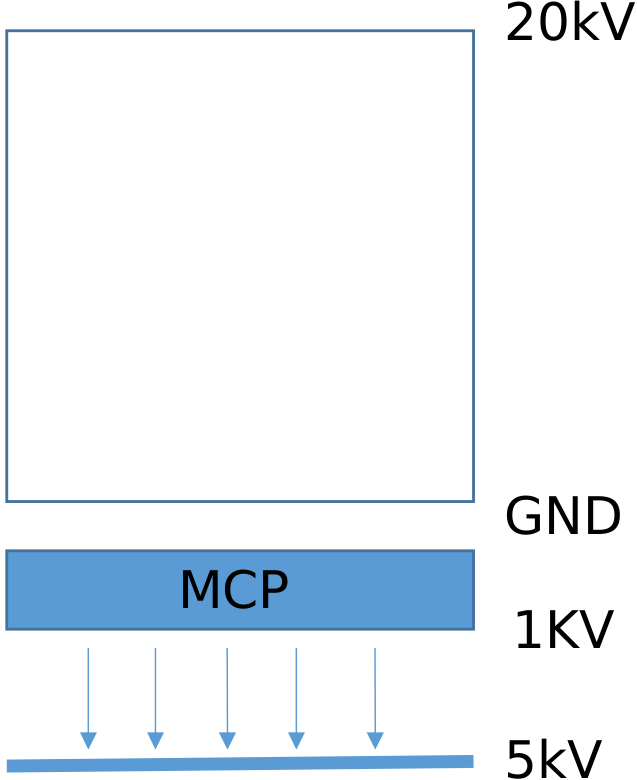
\includegraphics[width=0.7\textwidth]{04_IPHI_Test/figures/fig000_setup_hv_asym}
    \caption{Asymmetric configuration.
    Readout is grounded while extracting electrode is at a certain potential.}
    \label{chap4:setup_hv_asym}
  \end{subfigure}
  ~
  \begin{subfigure}[t]{0.5\textwidth}
    \centering
    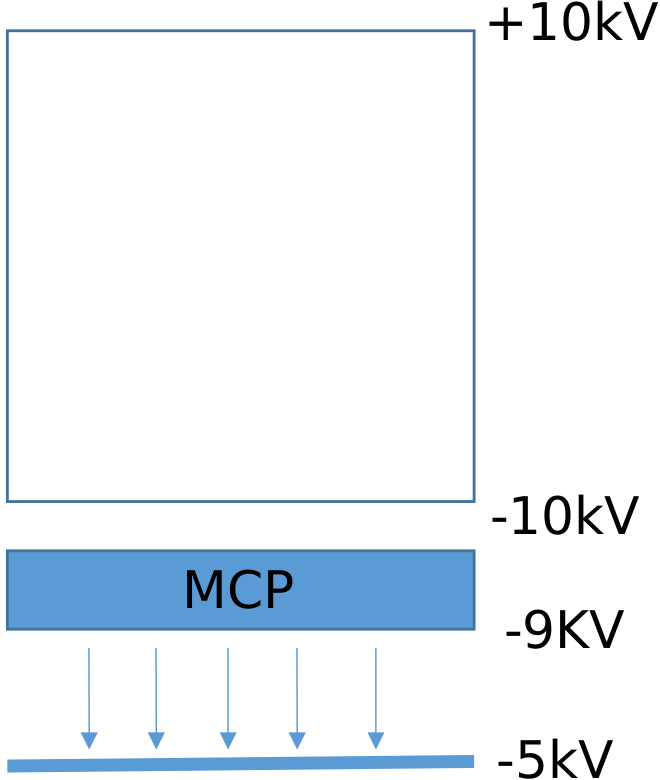
\includegraphics[width=0.7\textwidth]{04_IPHI_Test/figures/fig000_setup_hv_sym}
    \caption{Symmetric configuration. Readout and extracting electrode are at opposite potential.}
    \label{chap4:setup_hv_sym}
  \end{subfigure}
  \caption[Asymmetric or symmetric configuration]{Asymmetric or symmetric configuration, MCPs allow both.}
  \label{chap4:setup_hv}
\end{figure}
